\chapter{Geografické údaje}
\section{\textsc{Základné pojmy v geografii}}
\paragraph{}
V tejto podkapitole sa vysvetľujú pojmy týkajúce sa geografie, súvisiacej z GPS prístrojmi a súradnicami.
\paragraph{Súradnicový systém}
" je vzájomne jednoznačné zobrazenie medzi množinou bodov n-rozmerného priestoru
a usporiadanou n-ticou skalárov (veličín či čísiel; spravidla reálnych čísiel).
Tieto skaláre (pri ktorých záleží na poradí v ktorom sú uvádzané) sa nazývajú
súradnice alebo koordináty."[2]%" [Marián Jurík]
\paragraph{WGS-84}
\footnote{\textbf{WGS-84} - World Geodetic System 1984}
"WGS 84 je pravotočivá karteziánska sústava súradníc so stredom v ťažisku Zeme (vrátane morí a atmosféry). Kladná os x smeruje ku priesečníku nultého poludníka a rovníka, kladná os z ku severnému pólu a kladná os y je na obe predchádzajúce kolmá v smere doľava (90° východnej dĺžky a 0° šírky), tvorí tak pravotočivú sústavu súradníc"[12]

\begin{figure}[ht]
\centering
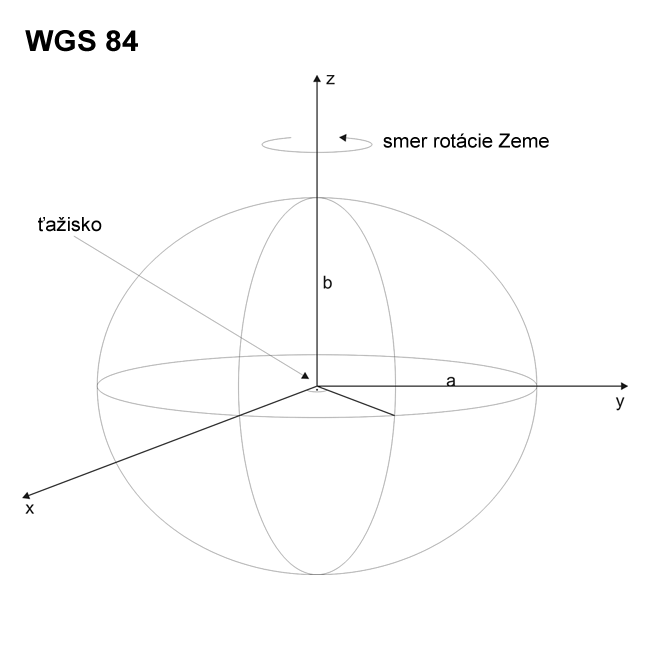
\includegraphics[height=9.0cm]{obr/Wgs84}
\caption{Systém udávania súradníc}
\end{figure}

\paragraph{}\paragraph{}\paragraph{}%\paragraph{}
\section{\textsc{Kartografická projekcia - Zobrazenie Máp}}
\paragraph{}
Prvoradý predpoklad analýzy a tvorby mapových výstupov z geografických
(vektorových\footnote{\textbf{Vektor} - prvok vektorového priestoru (na rozdiel od skaláru je okrem svojej absolútnej hodnoty určený aj smerom a orientáciou)} alebo rastrových\footnote{\textbf{rastrová grafika} - označuje spôsob uloženia grafickej informácie jednotlivých bodov usporiadaných v pomyslenej mriežke}) údajov je, že sa tieto údaje vzťahujú k jednotnému
súradni\-co\-vé\-mu systému (vysvetlený v predošlej kapitole).

Vo väčšine prípadov sú údaje z rôznych mapových podkladov, ktoré boli vyhotovené
v rôznych kartografických zobrazeniach a v rôznych mierkach. Nevyhnutnou
súčasťou procesu tvorby priestorovej databázy a mapových výstupov je preto
transformácia súradníc objektov medzi rôznymi súradnicovými systémami.
Pri spracovaní údajov berieme do úvahy min tri zobrazenia:
zobrazenie vstupných máp, interné zobrazenie (v programe), zobrazenie výstupov (dáta).
Ideálne je keď sa tieto zobrazenia zhodujú čo sa ale nestáva často.

\paragraph{}
\begin{figure}[ht]
\centering
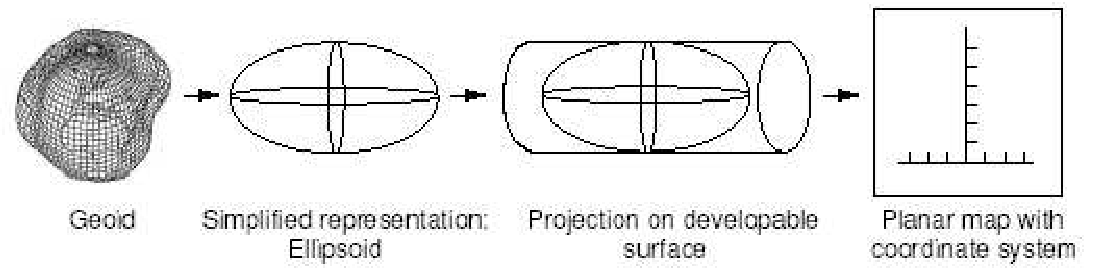
\includegraphics[width=14.5cm]{obr/zem_do_mapy}
\caption{Zpracovanie zemského povrchu do mapového zobrazenia}
\end{figure}

Význam interného kartografického zobrazenia, jednotného súradnicového systému a~presnosti kartografických transformácii rastie priamo úmerne s veľkosťou
spracová\-va\-né\-ho územia a s počtom užívateľov geografickej databázy. Pre
lokálne
databázy prístupne obmedzenému počtu užívateľov (napr. mapa zelene v intraviláne
jednej obce), postačuje zadefinovať lokálny pravouhlý súradnicový systém. Na
malých vzdialenostiach sa zakrivenie zemského povrchu môže zanedbať. Na
zjednotenie máp zelene všetkých obci okresu určite budeme potrebovať
transformáciu do jednotného su\-rad\-ni\-co\-vé\-ho systému. V prípade
medzinárodných
projektov, keď záujmové územie presahuje hranice jedného štátu a databázu
používajú organizácie z rôznych štátov s rôznymi národnými zobrazeniami a
tradíciami, sa vhodné riešenie hľadá ťažko.

\subsection{Referenčný elipsoid} 
Matematická aproximácia tvaru Zeme a iných telies vo vesmíre je referenčným elipsoidom. Skutočný tvar zeme je nepravidelný, no nejedná sa len o hory, kopce ale aj samotné moria sú nepravidelne vzdialené od stredu zeme (geoid viď. obrázok 1.3). Vplýva na to nepravidelné rozloženie hmoty zeme a tým aj rôznymi gravitačnými potenciálmi na zemi. Kľudová vzdialenosť hladiny mora sa môže líšiť na niektorých miestach zeme až o 100 metrov.

Základným súradnicovým systémom na referenčnom elipsoide sú \textbf{zemepisné
sú\-rad\-ni\-ce},
niekedy tiež nazývané geodetické zemepisné, alebo geografické sú\-rad\-ni\-ce.
Sú tvorené \textbf{zemepisnou (geografickou) šírkou a zemepisnou (geografickou) dĺžkou}. Zemepisné poludníky a
rovnobežky vytvárajú na referenčnom elipsoide zemepisnú sieť. Referenčný
elipsoid sa používa pri definícii štátnych a medzinárodných geodetických
súradnicových systémov, pri tvorbe mapových dielov veľkých a stredných mierok,
keď sa vyžaduje minimálne skreslenie.

\begin{figure}[ht]
\centering
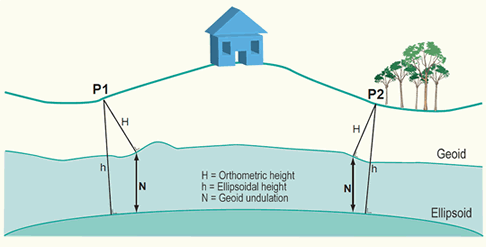
\includegraphics[width=14.5cm]{obr/relationshipse}
\caption{Referenčný elipsoid}
\end{figure}

\section{\textsc{GPS}}
\paragraph{}
"Global Positioning System, zvyčajne nazývaný GPS (armáda USA ho označuje ako
NAVSTAR GPS\footnote{\textbf{NAVSTAR GPS} - NAVigation Signal for Timing And Ranging}), je satelitný navigačný
systém používaný na zistenie presnej pozície a poskytujúci veľmi presnú časovú
referenciu takmer kdekoľvek na Zemi alebo na zemskom orbite. Používa zostavu
aspoň
24 satelitov na strednom zemskom orbite."[11].

Tento navigačný systém je funkčný 24 hodín denne, celý čas dokáže poskytovať údaje. Jedná sa o pasívny dĺžkomerný družicový systém. Cieľom tohto systému je poskytovať údaje o polohe na ktorej sa prijímateľ signálu nachádza. Pôvodne bol určený na vojenské účely, na zisťovanie polohy, rýchlosti a času. Neskôr ale americká vláda rozhodla o sprístupnení GPS signálu pre verejnosť. Systém je dostupný neustále vďaka tomu že jeho družice sú rozmiestnené tak aby v každom okamihu na celej zemi boli dostupné aspoň štyri satelitné prijímače. Štyri práve preto lebo tento signál sa vypočítava zo štyroch veličín (viď obr. 1.1) tieto veličiny sú hodnoty \textit{x,y,z} a posledná potrebná veličina je čas \textit{t}. V špeciálnych prípadoch nám postačujú aj tri veličiny a to vtedy keď máme jednu z veličín známu. Preto známu, lebo niektoré prístroje sú schopné zistiť nadmorskú výšku(pr. systémy na morských lodiach).

\paragraph{Konkurencia}
\begin{enumerate}
\item GLONASS\footnote{\textbf{GLONASS} - Globálny satelitný navigačný systém} - ruský družicový navigačný systém
\item Galileo - výstavbu realizuje Európska únia. Systém Galileo by mal byť prevádzkyschopný od roku 2010.
\item Compass - vyvíjaný Čínou, regionálne používaný pod názvom Beidou
\item DORIS - systém vyvíjaný Francúzskom
\end{enumerate}

\subsection{\textsc{Funkčnosť GPS systému}}
\paragraph{}
"To, čo sa deje v každom GPS prijímači by sme mohli opísať ako určovanie polohy
meraného bodu z priesečníku guľových plôch, ktorých polomer je daný meranými
vzdialenosťami. Tento systém sa nazýva tiež dĺžkomerný systém. Meranou veličinou
je doba šírenia rádiového signálu z družicovej antény k anténe GPS prijímača. Rýchlosť šírenia signálu je rovná rýchlosti svetla. Každá družica v
navigačnej správe okrem iných údajov posiela aj parametre svojej dráhy
z ktorých vieme vypočítať aktuálnu polohu družice (\textit{XS, YS, ZS}). Keď
poznáme súradnice družíc, môžeme polohu užívateľa (\textit{X, Y, Z}) určiť vypočítaním
sústavy troch rovníc o troch neznámych. Problém merania polohy by bol
jednoduchý, keby časové základne (hodiny) družice a užívateľa boli synchrónne.
Hlavný problémom je doba, ktorá uplynie medzi vyslaním diaľkomerného signálu z
GPS družice a jeho prijatím užívateľským GPS prijímačom. Časová základňa
užívateľského zariadenia je posunutá o neznámy časový interval \textit{Dt}, ktorý môžeme
prepočítať na vzdialenosť \textit{b = c Dt} (kde c je rýchlosť svetla). K neznámym
súradniciam užívateľa pristupuje teda neznáma \textit{b} a pre výpočet polohy potrebujeme
celkom štyri rovnice

\begin{verbatim}
(xi - x)2 + (yi - y)2 + (zi - z)2 = Di + b
Di = c tmi
i = 1, 2, 3, 4   "[11].
\end{verbatim}

\section{\textsc{Možnosti zobrazenia máp}}
\subsection{On-line mapy} 
\paragraph{}
Vo všeobecnosti majú veľké množstvo dát. Tieto mapy sú rozdelené na
množstvo fotografií ktoré sú kalibrované GPS súradnicami tak aby tvorili jeden
celok. Počet obrázkov na ktoré sú rozdelené je určený priblížením. Každý obrázok
má konštantnú veľkosť v pixloch. Mapy ktoré vidíme sú delené, na konštantnú
veľkosť. Čím je priblíženie väčšie tým je počet obrázkov väčší. Pri
pohľade na mapu vidíme, že približovaním sa zväčšuje detail na mape. Väčšina
užívateľov si pritom vôbec neuvedomí že priblížením sa pozerá na úplne inú
fotografiu = mapu rovnakú no z väčším počtom detailov. 
\paragraph{}
V súčasnosti máme možnosť výberu rôznych dostupných on-line máp. Medzi najznámejšie partia:
\begin{list}{•}
\item OpenStreetMap
\item
\item GoogleMaps
\item MapQuest
\item Yahoo! Maps
\item Multimap.com (Spojené kráľovstvo)
\item Map24
\end{list}

Každé majú svoje výhody aj nevýhody. V nasledujúcej podkapitole budú niektoré popísané.

\subsection{\textsc{Spôsob sťahovania konkrétnych častí mapy}}
\paragraph{}
Keďže mapu nemáme dostupnú celú, musíme pri pohybe priebežne sťahovať jednotlivé jej časti. Avšak je nutné vykonať istý numerický prepočet. Tento prepočet sa vykoná podľa
aktuálnej pozície GPS. Pri prepočte musíme zohľadniť priblíženie, veľkosť
obrázka a samotné súradnice.\\\\
Pri sťahovaní obrázka zo serveru zadávame do adresy tri hodnoty:
\begin{list}{•}
\item prepočítanú zemepisnú šírku
\item
\item prepočítanú zemepisnú dĺžku 
\item hodnotu priblíženia (zvyčajne hodnoty 2-17)
\end{list}

Dostupnosť maximálneho priblíženia určuje typ on-line mapy, rôzne on-line mapy
môžu mať rôzne priblíženie.

\subsection{\textsc{Google Mapy}}
\paragraph{Google maps}
 "je bezplatná, on-line mapová služba spoločnosti Google. Ponúka
posú\-va\-teľ\-né mapy a satelitné snímky celého sveta...

Označenie „satelitné snímky“ však nie je celkom presné, pretože časť záberov s
najväčším rozlíšením (prevažne z územia USA, ale aj napr. z Paríža) pochádza z
leteckého snímkovania."[5]

\subsubsection{Satelitná snímka} 
Tento pojem je vlastne fotografia fotená (snímaná) zo satelitu z výšky približne niekoľko tisíc metrov. Táto fotografia je následne spracovaná kalibráciou\footnote{\textbf{Kalibrácia} - je určenie presných súradníc kalibračných bodov} následne je možné mapu použiť na navigáciu príp. určenie polohy. Takýmito mapami disponuje aj spoločnosť Google, pod názvom "GoogleMaps".\\\\\\

Satelitné snímky existujú v dvoch typoch:
\begin{enumerate}
\item Snímky s komerčného satelitu QuickBird, ktoré sú schopné snímať plochu o rozmeroch (16,5 x
16,5) km. Maximálne rozlíšenie týchto snímok je 60 cm na pixel\footnote{\textbf{pixel} - skratka z angl. picture element - obrazový prvok} (viď. obrázok 1.4). Počas jedného snímania je satelit schopný spojiť až 10 snímok čím vznikne výsledný snímok o veľkosti (16,5 x 165) km 

\item Snímky z Amerického programu Landsat, ktorý pracuje od roku 1972. Najnovší satelit, ktorý pracuje v rámci tohto programu je Landsat 7. Tento satelit je schopný snímať maximálnu plochu o rozmeroch (185 x 185) km. Pracuje s rozlíšením 15 m na pixel. Zem je takto neustále snímaná až do súčasnosti.
\end{enumerate}

\begin{figure}[ht]
\centering
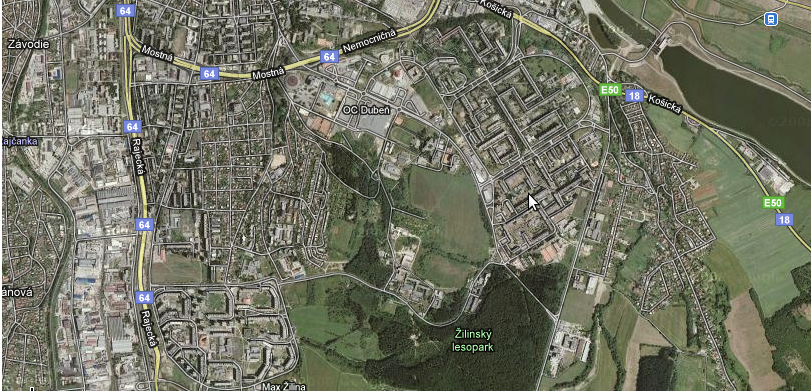
\includegraphics[width=14.5cm]{obr/gogmaps}
\caption{Príklad zobrazenia Google Máp}
\end{figure}

\subsection{\textsc{OpenStreetMap}}
\paragraph{OpenStreetMap(OSM)}
  "je otvorený projekt, ktorého cieľom je tvorba voľných
geografických dát, ako sú napríklad cestné mapy. Používa predovšetkým dáta z
prijímačov GPS (v režime automatického zaznamenávania súradníc prechádzanej
trasy), ktoré sú následne kontrolované a editované. Je založený na kolektívnej
spolupráci a na koncepcii Open source\footnote{\textbf{Open source} - voľne šíriteľný}."[9].

Tvorba máp a zaznamenávanie ciest do máp sa dá považovať za úspešné vzhľadom na to, že počet používateľov týchto máp stále stúpa. Značne množstvo ľudí láka hlavne to že do tvorby máp sa môžu zapojiť a tak si môžu vytvárať mapy svojho okolia, ktoré následne môže využiť ktokoľvek. OpenStreetMap je nezisková organizácia, ktorej zakladateľ je Steve Coast. Ako organizácia sa tento projekt označuje od roku 2006. Všetky tieto dáta je možné upravovať používateľmi máp. Nato aby sme mohli dáta do databázy nahrávať a aby sa mohli neskôr porovnať je potrebné sa zaregistrovať na stránke \url{http://www.OpenStreetMap.org}. \\
Slovenská stránka pre OSM je \url{http://www.freemap.sk/}


\paragraph{Šírka záberu} Mapovacie rozhranie zhŕňa síce celý svet ale hlavné body pre mapovanie sa odohrávajú vo Francúzku, Škandinávii, na ostrove Man a v Spojenom kráľovstve. Dáta z územia USA pochádzajú z databázy TIGER\footnote{\textbf{TIGER} - vytvorené pri sčítaní ľudu}. 

\begin{figure}[ht]
\centering
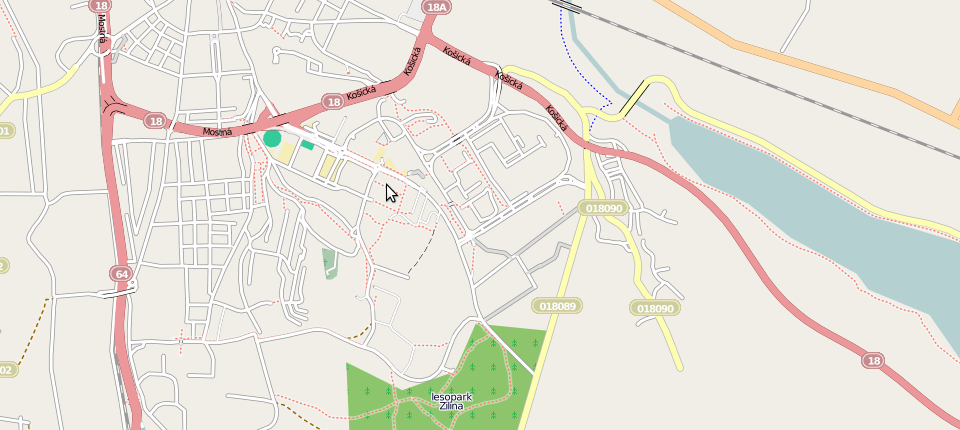
\includegraphics[width=14.5cm]{obr/osm}
\caption{Príklad zobrazenia Open Street Map}
\end{figure}

\paragraph{Zdroj dát} nie sú ako by sme možno očakávali z konkrétnej firmy alebo organizácie, ale od bežných používateľov ktorý si svojvoľne snímajú dané trasy. Tieto trasy následne prejdú analýzou a po zhodnotení (porovnaní so satelitnými snímkami družice Landsat7) sa dané trasy zapíšu do mapy. Týmto spôsobom je zaistený ich skutočný stav ich umiestnia.
